\section{Punto de Vista Estructura de Información}
Una estructura de información es una estructura jerárquica centrada en el producto que organiza la información relacionada con un producto o biblioteca. Dentro de una estructura de información, los subgrupos de información denominados grupos de información organizan el contenido. Estos objetos de contenido se denominan elementos de información. Los criterios de filtro ofrecen la posibilidad de identificar y administrar la información asociada a las variaciones del producto. Las estructuras de información se pueden filtrar para mostrar componentes opcionales o artículos con valores de atributo específicos. Los objetos se muestran en la estructura según el filtro de la estructura actualmente activo. Se pueden editar los filtros y renovar la estructura para mostrar los objetos que cumplen con los nuevos criterios de filtro. Las estructuras de información se pueden comparar para determinar el impacto de los cambios en el producto. La estructura de información que se encuentra actualmente en producción se puede comparar con una nueva estructura de información bajo desarrollo para revelar el impacto de los cambios propuestos. Las relaciones con la información de producto de soporte permiten determinar la cantidad y el ámbito del trabajo que se va a hacer.

\subsection{Modelo de Estructura de Información}
\begin{figure}[h!]
	\centering
	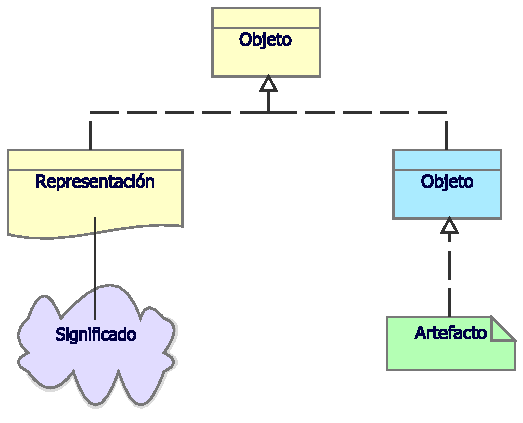
\includegraphics[width=.62\linewidth]{imgs/modelo/EstrInformacion}
	\caption{Modelo Estructura de Información}
\end{figure}

Esta quinta sección de puntos de vista llamada tecnología en la cual se involucra todo lo concerniente a la parte tecnológica, su uso, la implementación y el despliegue, la parte física, las capas, el servicio y la estructura de la información del proyecto, este último punto de vista de la estructura de información está compuesto por cinco elementos principalmente, tal y como se muestra en el diagrama anterior del modelo. Estos elementos son: como principal, está el objeto y el objeto secundario, luego se deriva en una representación y significado del mismo y por la parte de los objetos se desprende un artefacto por medio de una realización. 


\subsection{Caso  de Estructura de Información}
\begin{figure}[h!]
	\centering
	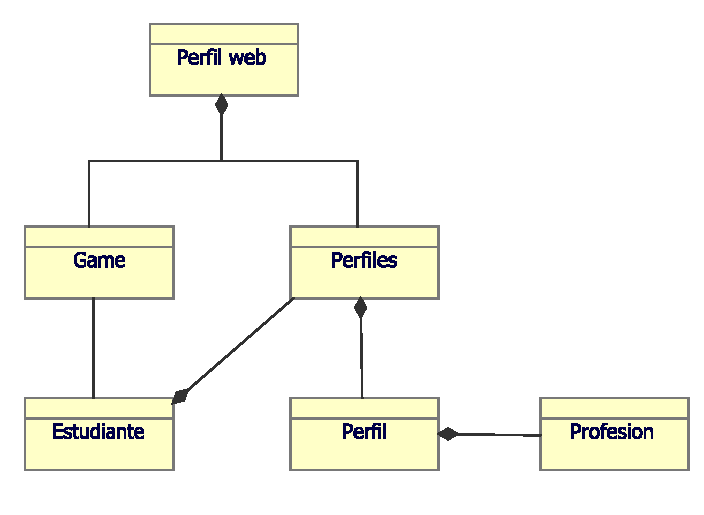
\includegraphics[width=.8\linewidth]{imgs/caso/estructuraInformaci}
	\caption{Caso Estructura de Información}
\end{figure}

El punto de vista de la estructura de la información es comparable a los modelos de información tradicionales creados en el desarrollo de casi cualquier sistema de información. Muestra la estructura de la información utilizada en la empresa o en un proceso de negocio o aplicación específicos, en términos de tipos de datos o estructuras de clases (orientadas a objetos). Además, puede mostrar cómo la información a nivel empresarial se representa en el nivel de la aplicación en la forma de las estructuras de datos que se utilizan allí, y cómo se asignan luego a la infraestructura tecnológica subyacente, destacando que es un enfoque de muy alto nivel hacia por ejemplo, por medio de un esquema de base de datos, tal y como se realizó para el proyecto Tu-Perfil en donde se tiene el objeto de negocio llamado Perfil Web y una serie de elementos o entidades importantes a tener en cuenta para modelar como los perfiles que tiene un perfil para una profesión y lógicamente el estudiante a perfilar, sin dejar de lado la parte del juego o Game que realiza la función de brochure para la base de datos.

\clearpage